\documentclass[12pt]{article}
%\documentclass{nature}

% Including pdf figures
\usepackage{graphicx}
\graphicspath{ {../Plots/} }
\usepackage{pdfpages}
%really place a figure in a location
\usepackage{float}
%Overrun caption
\usepackage[CaptionAfterwards]{fltpage}
% Math stuff
\usepackage{amsmath}
% Bibliographies
\usepackage[numbers]{natbib}
\bibpunct{(}{)}{,}{a}{}{;} 

\usepackage[font={scriptsize}]{caption}

\usepackage{lineno} %gives line numbers with \lineno command

\usepackage{setspace}
\onehalfspace

\begin{document}

\title{Gametic Selection, Sex Ratio Bias, and Transitions Between Sex Determination Systems}
\author{Michael F Scott$*^1$ and Matthew M Osmond$*^2$, and Sarah P Otto$^2$}
\date{}
\maketitle
\noindent
$*$ These authors contributed equally to this work

\noindent
$^1$ Department of Botany, University of British Columbia, \#3529 - 6270 University Boulevard, Vancouver, BC, Canada V6T 1Z4

\noindent
$^2$ Department of Zoology, University of British Columbia, \#4200 - 6270 University Boulevard, Vancouver, BC, Canada V6T 1Z4

\noindent
email: mfscott@biodiversity.ubc.ca, mmosmond@zoology.ubc.ca

\noindent
Contributions: 

\newpage
\linenumbers
\modulolinenumbers[2]

\begin{abstract}
Sex determination systems are remarkably dynamic; many studied taxa display transitions of sex-determining genes between chromosomes or the evolution of new sex-determining systems. 
%Predominant theories in which new sex-determining systems are favoured by selection involve sex ratio selection or fitness differences between sexes (e.g., sexually antagonistic selection). 
Here, we utilize population genetic models to study the spread of novel sex-determiners in systems with 
%a period of selection during the haploid stage produced by one sex, e.g., pollen or sperm competition. 
haploid gametic selection, e.g., pollen or sperm competition.
Haploid selected loci experience a form of sex-specific selection (because gametic competition occurs predominantly among haploids produced by males) and can cause sex ratios at birth to become biased (because sex ratios are determined by the fertilization success of X- versus Y-bearing pollen/sperm). 
%We find that the evolution of sex determination systems where mothers determine sex at birth (e.g., environmental sex determination where sex is determined at birth) is influenced by classic Fisherian sex ratio selection. {\color{red}(Maybe not true???)}
%However, notably, we find that the spread of new genetic sex determination systems is not affected by sex ratio biases that are caused by gametic selection because sex ratios become biased after parental provisioning has occurred (even if pollen/sperm competition occurs within the mother). 
Notably, we find that the spread of new genetic sex determination systems is not affected by sex ratio biases that are caused by gametic selection because sex ratios become biased after parental provisioning has occurred (even if pollen/sperm competition occurs within the mother). 
In addition, we find that linkage of an ancestral sex chromosome to a locus under haploid selection can favour transitions between male and female heterogamety (e.g., XY to ZW), which is not the case for any forms of diploid sex specific selection (e.g., sexually antagonistic selection).
During these transitions, new sex-determining alleles spread despite breaking up favourable associations that build up between ancestral sex-determining loci and selected loci, reducing population mean fitness. 
Furthermore, a period of selection among haploids can favour the stable maintenance of polymorphic sex determination systems. 
Thus, our models offer several new insights to be explored as information about sex determination in non-model taxa accumulates.

%[Approx 320 words]
\end{abstract}

\newpage

\section*{Introduction}

%CHECK THROUGHOUT: use of sex-determination SYSTEMS versus MECHANISMS. 

Animals and angiosperms exhibit extremely diverse sex determination systems \citep[reviewed in][]{Bull:1983vi,Charlesworth:2010it,Beukeboom:2014vb,Bachtrog:2014bx}. 
Among species with genetic sex determination of diploid sexes, some taxa have heterogametic males (XY) and homogametic females (XX), including %non-monotreme? 
mammals and most dioecious plants \citep{Ming:2011iy}; whereas other taxa have homogametic males (ZZ) and heterogametic females (ZW), including Lepidoptera and birds. 
Within several taxa, the chromosome that harbours the master sex-determining region changes. 
For example, transitions of the master sex-determining gene between chromosomes or the evolution of new master sex-determining genes have occurred in Salmonids \citep{Li:2011fm,Yano:2012di}, Diptera \citep{Vicoso:2015hf}, and \textit{Oryzias} \citep{Myosho:2012fv}.
%Presentation at evolution found neo sex chromosome in birds, doesn't seem to be published or bioRxiv yet (consider pers com.), title: A previously unknown neo-sex chromosome mediates plumage divergence and speciation in hybridizing birds Jason Sardell; Elizabeth Cooper; J. Albert C. Uy. I wonder if this is actually a fusion event though?
In addition, many gonochoric/dioecious clades with genetic sex determination exhibit transitions between male (XY) and female (ZW) heterogamety, including lizards \citep{Ezaz:2009tk}, eight of 26 teleost fish families \citep{Mank:2006bt}, true fruit flies \citep[Tephritids,][]{Vicoso:2015hf}, amphibians \citep{Hillis:1990gu}, the angiosperm genus \textit{Silene} \citep{Slancarova:2013dq}, Coleoptera and Hemiptera \citep[][plate 2]{Beukeboom:2014vb}.
Indeed, in some cases, both male and female heterogametic sex determination systems can be found in the same species, as exhibited by some cichlid species \citep{Ser:2010iq} and \textit{Rana rugosa} \citep{Ogata:2007jm}.
In addition, multiple transitions have occurred between genetic and environmental sex determination systems, e.g., in reptiles and fishes \citep{Conover:1987in,Mank:2006bt,Pokorna:2009ui,Ezaz:2009tk,Pen:2010kk,Holleley:2015hc}.

%NOTE: ``Bull & Charnov (1977) hypothesized that a new sex-determining gene can rapidly increase and become fixedin a population if it is linked to a gene with high adaptivevalue, and finally cause a change of the heterogametic sex.'' The Bull and Charnov paper is also the one in which the set of neutral equilibria between XY and ZW are identified (where sex ratios are equal)
%NOTE: Vuilleumier et al. 2007 also find polymorphic sex determination can be stable.

%For example, closely related species in the Medaka lineage (cite Takenhana et al. 2008) and Tilapiinae (cite Lee et al 2004, Cnaani et al 2008), citations in Beukeboom. 

%\textcolor{red}{Brief description of sex ratio adjustment and sexual antagonism theories:}

Predominant theories in which new sex determination systems are favoured by selection involve fitness differences between sexes (e.g., sexually antagonistic selection) or sex ratio selection.
%\citet{Bull:1977wt} shows that direct selection on new sex determination loci can allow them to spread and switch between male and female heterogamety. 
\citet{vanDoorn:2007eu,vanDoorn:2010hu} show that new sex determination loci can be favoured if they arise in close linkage with a locus that experiences sexual antagonism. 
For example, linkage allows favourable associations to build up between a male-beneficial allele and a neo-Y chromosome. 
Such associations can favour a new master sex-determining gene on a new chromosome \citep{vanDoorn:2007eu} and can also favour a transition between male and female heterogamety \citep[e.g., a ZW to XY transition,][]{vanDoorn:2010hu}.
However, any sexually-antagonistic loci that are linked to the ancestral sex-determination locus will develop similar, favourable associations and select against the spread of a new sex-determination system. 

It has been suggested that sex ratio selection could be a particularly important force driving transitions between sex-determining systems \citep[Chapter 7]{Beukeboom:2014vb}. 
For example, flexible sex determination systems may be favoured in order to exploit local environmental conditions that are optimal for males or females, which creates locally biased sex ratios \citep{Charnov:1977tx,Werren:1984tl,Pen:2010kk}. 
In addition, feminizing mutations may invade when female biased sex ratios are favoured due to selection among demes \citep{Wilson:1981vm,Vuillleumier:2007bh}. 
In other situations, sex ratio selection may favour transitions in order to restore equal sex ratios. 
For example, \citet{Kozielska:2010vm} consider systems in which the ancestral sex chromosomes experience meiotic drive (e.g., where driving X or Y chromosomes are inherited disproportionately often), which causes sex ratios to become biased \citep{Hamilton:1967ts}. 
They find that new, unlinked sex-determining loci (masculinizing or feminizing mutations, i.e., neo-Y or neo-W loci) can then spread, restoring an even sex ratio. 

%\textcolor{red}{We add haploid selection:}

Here, we use mathematical models to find the conditions under which new sex determination systems are favoured by selection when there is a period of selection among haploid gametes/gametophytes. 
Selection among haploid genotypes is thought to occur primarily among pollen/sperm, which can compete whenever there are more pollen/sperm than required for fertilization \citep{Mulcahy:1996ha,JOSEPH:2004haa}. 
Haploid selection may be particularly common in plants, in which 60-70\% of all genes are expressed in the male gametophyte and these genes exhibit stronger signatures of selection than random genes \citep{Borg:2009jpa,Arunkumar:2013iq,Gossmann:2014dua}.
In addition, artificial selection pressures applied to male gametophytes cause the frequency of resistant alleles to increase \citep[e.g.,][]{Hormaza:1996cv,Ravikumar:2003uo,Hedhly:2004iv,Clarke:2004ir}. 
A smaller (but non-negligible) proportion of genes are thought to be expressed and selected in animal sperm, although precise estimates are uncertain \citep{Zheng:2001fi,JOSEPH:2004haa,Vibranovski:2010et}.
\textcolor{red}{add something about meiotic drive here?}  

There are various ways in which a period of haploid selection could influence transitions between sex determination systems. 
Firstly, if we assume that haploid selection at any particular locus predominantly occurs in one sex (e.g., pollen/sperm competition), then such loci experience a form of sex-specific selection. 
In this respect, we might expect that haploid selection might affect transitions between sex determination systems in a similar manner to sex-specific diploid selection \citep[as explored by][]{vanDoorn:2007eu,vanDoorn:2010hu}. 
That is, new masculizing mutations (neo-Y chromosomes) could be favoured via linkage associations with alleles that are beneficial in pollen/sperm. 
However, sex ratios can also become biased if there is linkage between the sex-determining region and a locus that harbours genetic variation in haploid fitness. 
For example, differences in fitness between X- and Y-bearing pollen tubes can cause the sex ratio among seeds to become biased when there is pollen competition \citep{Lloyd:1974tz,Conn:1981uw,Stehlik:2005ul,Stehlik:2006to,Field:2012fd,Field:2013cc}.
It is not immediately clear how the spread of new sex determination systems would be influenced by the combination of sex ratio biases and favourable associations between haploid selected loci and sex-determining regions. 

Surprisingly, our models show that haploid selection influences the evolution of new sex determination systems in a way that is distinct from both diploid sex-specific selection and sex ratio selection. 
We find that new genetic sex determination systems are not affected by any sex ratio biases caused by associations between sex-determining regions and haploid selected loci. 
In addition, we find that associations that build up between an ancestral sex-determining locus and a haploid-selected locus can favour transitions between male and female heterogamety (e.g., a neo-W allele arising at a previously autosomal locus spreads in an ancestrally XY system), despite the fact that these ancestral associations were built up by selection. 
This does not occur in models that do not include haploid selection. 

\textcolor{red}{NOTE RE: DRIVE. I expect drive (that occurs specifically in one sex, e.g., during spermatogenesis) to behave almost exactly like haploid selection. That is, I think that a XY-linked driver that is maintained by selection (e.g., because it causes sterility when homozygous, which is common in known drive systems) will only favour invasion of a more tightly linked neo-Y (worsening sex ratio biases) and could favour invasion of a neo-W. This may run counter to generic expectations from new sex chromosome systems evolving to balance the sex ratio. So, do you think it would significantly enhance the paper to model drive explicitly or just discuss it as being similar???}

{\color{blue} 
FOR RESULTS?

FROM PREVIOUS PAPER:
The maintenance of polymorphism at loci that experience sex specific selection in both haploid and diploid phases was considered by Immler et al. \cite{Immler:2012tl}, demonstrating that polymorphisms can be maintained by sexually antagonistic selection or overdominance as well as by conflicting selection pressures in haploids and diploids (haploid-diploid conflict or ploidally antagonistic selection) or a combination of these selective regimes.  
}


%%%%%%%%%%%%%%%%%%%%%%%%%%
\section*{Model}
%%%%%%%%%%%%%%%%%%%%%%%%%

%genetic system
We consider a three locus model.
Locus \textbf{X} is the ancestral sex-determining region, with alleles $X$ and $Y$ (or $Z$ and $W$).
Locus \textbf{A} is a region under selection, with alleles $A$ and $a$.
And locus \textbf{M} is a novel sex-determining region, with alleles $M$ and $m$.
With genotype $MM$ at locus \textbf{M}, the sex of a zygote is determined by the genotype at locus \textbf{X} ($XX$ become females and $XY$ become males, or $ZW$ become females and $ZZ$ become males).
With at least one $m$ allele at locus \textbf{M}, a zygote develops as a female with probability $k$ and as a male with probability $1-k$.
With $k=0$, the novel sex determiner is a masculinizer (i.e., a neo-Y) and with $k=1$ the novel sex determiner is a feminizer (i.e., a neo-W).
With intermediate $k$, locus \textbf{M} is interpreted as an offspring controlled environmental sex-determining region.
Finally, we also analyze a model of maternally-controlled environmental sex-determination (ESD), where mothers with at least one $m$ allele produce daughters with probability $k$. 

%life-cycle
The life-cycle begins with competition between haploid gametes/gametophytes (hereafter gametes) from each sex, where selection depends on the sex of the diploid they came from and their allele at the \textbf{A} locus.
Gametes from males then pair randomly with gametes from females.
The resulting zygotes develop as males or females, depending on their genotypes at the \textbf{X} and \textbf{M} loci (and the \textbf{M} genotype of their mother in the case of maternal control).
Diploids compete with others of the same sex, where selection depends on the sex of the individual and its genotype at the \textbf{A} locus.
This is followed by meiosis with recombination and sex-specific meiotic drive. 
Recombination occurs between loci \textbf{X} and \textbf{A} with probability $r$, between loci \textbf{A} and \textbf{M} with probability $R$, and between loci \textbf{X} and \textbf{M} with probability $\chi$. %is chi really the prob of rec in our recursion equations?
Any order of the loci can be modelled with appropriate choices of $r$, $R$, and $\chi$.
We model meiotic drive at the viability locus only; individuals of sex $i$ who are heterozygous at the \textbf{A} locus produce haploids bearing allele $A$ with probability $\alpha^i$.
We track the frequency of haploid genotypes produced by each sex from one generation to the next (recursion equations in Sup.\ Mat.).

%what were going to do, briefly
With allele $M$ fixed at the \textbf{M} locus, sex is determined by locus \textbf{X} and an equilibrium is reached at locus \textbf{A}. %where, importantly, locus \textbf{A} can be stably polymorphic. %the dynamics can be described by the frequency of $A$ in gametes/gametophytes from the homogametic sex and the frequencies of $A$ in the two types of gametes/gametophytes from the heterogametic sex.
We then examine the ability of a rare, novel sex-determiner, $m$, to increase in frequency from this equilibrium.
Numerical simulations are used to examine when an invading mutation goes to fixation.

%%%%%%%%%%%%%%%%%%%%%%%%%%
\section*{Results}
%%%%%%%%%%%%%%%%%%%%%%%%%

\subsection*{Resident equilibrium and stability}
With allele $M$ fixed, we follow the dynamics of the frequency of $A$ in gametes from the homogametic sex (e.g., in eggs from an XX female, $p^f_X$), the frequencies of $A$ in the two types of gametes from the heterogametic sex (e.g., in sperm from an XY male that are X-bearing, $p^m_X$, and Y-bearing, $p^m_Y$), and the frequencies of the sex-determining factors in gametes from the heterogametic sex (e.g., the frequency of Y in sperm, $q$).
Assuming selection and meiotic drive are weak relative to recombination, the differences in the frequencies of $A$ in each type of gamete are small, as is the bias in the sex-determining factor from the heterogametic sex, and we can solve for the mean frequency of $A$ across all types ($p_A$), the difference in the frequencies of $A$ between two of the three types, and the bias in the frequency of the sex-determining factor, to first order in selection.
Linear stability analysis can then be used to determine the stability of this equilibrium.
Without haploid selection or meiotic drive our results reduce to those of \cite{vanDoorn:2007eu}. %when $k=0$ (neo-$Y$ invading a $ZW$ system) or when $k=1$ (neo-$W$ invading an $XY$ system) (\textcolor{red}{CHECK}).
However, with haploid selection or meiotic drive a stable polymorphism at locus \textbf{A} no longer requires sexually antagonistic selection. %, as it can also be achieved by ploidally-antagonistic selection.

\subsection*{Sex chromosome turnover}
The spread of a rare mutant $m$ at the \textbf{M} locus in such a population is determined by the leading eigenvalue, $\lambda$, of the system described by the equations for the next generation frequency of haploid genotypes with the mutation. %, evaluated at the above equilibrium.
Below we present the analytic results for invasion into an $XY$ system assuming no competition among gametes from females, no meiotic drive in females, and linear arrangement \textbf{X}\textbf{A}\textbf{M}. %(i.e., $\chi = r R$). %(SAY SOMETHING HERE ABOUT OTHER ARRANGEMENTS?). %equal dominance coefficients in the two sexes,
Equivalent results for invasions into a $ZW$ system are derived by consistently switching the roles of males and females. %\citep{vanDoorn:2010hu}.


%\subsubsection*{Neo-$Y$}
%
%%write in general form without weak selection
%A rare, dominant neo-$Y$ ($k=0$) is always expected to invade the ancestral $XY$ system when the average growth rate of mutant haplotypes ($Am$ and $am$) is positive, $(g_A + g_a)/2 > 0$. %($g_i = where $\lambda_i$ are the two eigenvalues when $R=r=0$; the \textbf{X} locus does not affect the dynamics).
%When the growth rates of the mutant haplotypes without recombination ($R=0$) are negative, $g_i^* < 0 \; \forall \; i \in \{A,a\}$, where $g_i < g_i^*$, the neo-$Y$ does not invade.
%Otherwise, the mutant allele increases in frequency on one \textbf{A} background and declines on the other and neo-$Y$ invasion requires
%\begin{equation}
%R \left[ \frac{p^f_X w_{m,a}}{g_A^*} + \frac{(1 - p^f_X) w_{m,A}}{g_a^*} \right] w_{m,Aa} < \nu_m,
%\end{equation}
%where $w_{m,i}$ is the relative viability fitness of males depending on their haploid or diploid genotype at the \textbf{A} locus (with $i\in\{A,a,AA,Aa,aa\}$) and
%$\nu_m = 
%  p^f_X p_{Ym} w^m_{a} w^m_{AA} +
%  p^f_X (1-p_{Ym}) w^m_{a} w^m_{AA} +
%  (1-p^f_X) p_{Ym} w^m_{a} w^m_{AA} +
%  (1-p^f_X) (1-p_{Ym}) w^m_a w^m_{AA}$
%is the mean relative fitness of resident males.
%%and $g_j^*$ is the growth rate of $X^m$ and $Ym$ haplotypes when on an $A$ ($j=A$)  or $a$ background ($j=a$).
%Neo-$Y$ invasion therefore occurs for any recombination rate, $R$, when the net flow of double recombinants is from the less fit to the more fit \textbf{A} background (making the term inside the square brackets negative).
%%Assuming $g_A^* > 0$ and $g_a^* < 0$ without loss of generality, this is $-(1 - p^f_X) w_{m,A} g_a^* < p^f_X w_{m,a} g_A^*$.
%When the net flow of double recombinants is from the more fit to the less fit haplotype, neo-$Y$ invasion can still occur when the rate of recombination is small enough.
%
%%weak selection
%Assuming weak selection, we can solve for the invasion fitness of the neo-$Y$ explicitly, giving
%\begin{equation}
%\lambda_{Y,XY} \approx 1 + V_A S_A (r - R)s^f,
%\end{equation}
%where $V_A = p_A(1-p_A)$ is the variance at the \textbf{A} locus, $S_A = s^f/ \left[ r R \left( s^f + s^m \right)^2 t_m^2 \right]$ (INTERPRETATION), $s^f$ and $s^m$ are the respective selection coefficients for $A$ in diploid females and males, $t_m$ is the selection coefficient for $A$ in gametes/gametophytes from males, and we've assumed equal dominance coefficients in the two sexes.
%The neo-$Y$ can therefore invade whenever it is in tighter linkage with the selected locus than the ancestral sex-determining locus, $r>R$, provided locus \textbf{A} is polymorphic ($V_A>0$) and there is selection among both females ($s^f\neq0$) and gametes/gametophytes from males ($t_m\neq0$).
%
%\subsubsection*{Neo-$W$}
%
%%write in general form without weak selection
%Similarly, a rare, dominant neo-$W$ ($k=1$) will invade the ancestral $XY$ system whenever the average growth rate of $XAm$ and $Xam$ haplotypes is positive, $(g_A + g_a) / 2 > 1$. 
%When the growth rates of the mutant haplotypes without recombination ($R=0$) are negative, $g_i^* < 0 \; \forall \; i \in \{A,a\}$, where $g_i < g_i^*$, the neo-$W$ does not invade.
%Otherwise neo-$W$ invasion requires
%\begin{equation}
%R \left[ \frac{\bar{p}_m w_{m,A}}{g_a^*} + \frac{(1 - \bar{p}_m) w_{m,a}}{g_A^*} \right] w_{f,Aa} < \nu_f
%\end{equation}
%where $\bar{p}_m = (p_{Ym}+p^m_X) / 2$ is the mean frequency of $A$ in gametes/gametophytes from males, $w_{f,i}$ is the relative viability fitness of females depending on their diploid genotype at the \textbf{A} locus (with $i\in\{AA,Aa,aa\}$), and 
%$\nu_f = 
%  p^f_X p^m_X w^m_{a} w_{AA,f} +
%  p^f_X (1-p^m_X) w^m_{a} w_{Aa,f} +
%  (1-p^f_X) p^m_X w^m_{a} w_{Aa,f} +
%  (1-p^f_X) (1-p^m_X) w^m_a w_{aa,f}$
%is the mean relative fitness of resident females. 
%%The rate of recombination between the \textbf{X} and \textbf{A} loci, $r$, does not explicitly appear because females are homozygous at the \textbf{X} locus with an ancestral $XY$ system.
%As in the case of the neo-$Y$, neo-$W$ invasion therefore occurs with any recombination rate, $R$, when the net flow of recombinants is from the less fit to the more fit haplotype.
%%Assuming $g_A^*>0$ and $g_a^*<0$ without loss of generality, this is $(1 - \bar{p}_m) w_{m,a} g_a^*< \bar{p}_m w_{m,A} g_A^*$.
%And when the net flow of recombinants is from the more fit to the less fit  haplotype, neo-$W$ invasion can still occur when the rate of recombination is small enough.
%
%%weak selection
%Assuming weak selection, we can solve for the invasion fitness of the neo-$W$ explicitly, giving
%\begin{equation}
%\lambda_{W,XY} \approx 1 + V_A S_A \frac{(2r(1-R)-R) s^f + (1-2r)R s^m }{2},
%\end{equation}
%where we've once again assumed equal dominance coefficients in the two sexes.
%In this case, even when the novel sex-determining locus is in looser linkage with the selected locus than is the ancestral sex-determining locus, $r<R$, a novel sex-determiner can invade.
%For example, with $R=1/2$ the neo-$W$ invades if there is any linkage between the ancestral sex-determining and selected loci ($r<1/2$), there is selection among gametes/gametophytes in males ($t_m\neq0$), and there is selection for or against $A$ in both males and females ($s^m s^f >0$) that is stronger in females than in males ($|s^f| > |s^m|$).

\subsubsection*{Neo-$Y$ and neo-$W$}

%<<<<<<< HEAD
%\subsubsection*{Neo-$Y$}
%
%The growth rate of a rare, dominant neo-$Y$ region ($k=0$) is
%\begin{equation}
%\lambda_{Y,XY} = 1 + V_A \frac{(r - R)}{r R} \frac{s_f^2}{\left( s_f + s_m \right)^2} t_m^2,
%\end{equation}
%where $V_A = p_A(1-p_A)$ is the variance at the \textbf{A} locus, $s_f$ and $s_m$ are the respective selection coefficients for $A$ in diploid females and males, and $t_m$ is the selection coefficient for $A$ in gametes/gametophytes from males.
%The neo-Y can therefore invade whenever it is in tighter linkage with the selected locus than is the ancestral sex-determining locus, $r>R$, provided locus \textbf{A} is polymorphic ($V_A>0$) and there is selection among both females ($s_f\neq0$) and gametes/gametophytes from males ($t_m\neq0$).
%=======
%>>>>>>> c89cd9e1d25a76e5bffdd1ee7574884f24c08070
%write in general form without weak selection
A rare, dominant neo-$Y$ ($k=0$) or neo-$W$ ($k=1$) is always expected to invade an ancestral $XY$ system when the average growth rate of the mutant haplotypes ($Am$ and $am$) is positive, $(g_A + g_a)/2 > 0$. %($g_i = where $\lambda_i$ are the two eigenvalues when $R=r=0$; the \textbf{X} locus does not affect the dynamics).
When the growth rates of the mutant haplotypes without recombination ($R=0$) are negative, $g_i^* < 0 \; \forall \; i \in \{A,a\}$, where $g_i < g_i^*$, the new sex-determining allele does not invade.

Otherwise, the new sex-determining allele increases in frequency on one \textbf{A} background and declines on the other, and invasion requires
\begin{equation}\label{eq:neoYR}
R \left[ \frac{p^f_X w^m_a (1-\alpha^m)}{g_A^*} + \frac{(1 - p^f_X) w^m_A \alpha^m}{g_a^*} \right] w^m_{Aa} < \nu^m,
\end{equation}
for the neo-$Y$, and 
\begin{equation}\label{eq:neoWR}
R \left[  \frac{(1 - \bar{p}^m) w^m_{a}}{g_A^*} + \frac{\bar{p}^m w^m_{A}}{g_a^*} \right] w^f_{Aa} < \nu^f
\end{equation}
for the neo-$W$.
Here $\bar{p}^m = (1-q) p^m_X+ q p^m_Y$ is the average frequency of $A$ in gametes produced by males, $w^i_{j}$ is the relative viability fitness of sex $i\in\{m,f\}$ depending on their haploid or diploid genotype at the \textbf{A} locus (with $j\in\{A,a,AA,Aa,aa\}$) and
$\nu^i = 
  p^f_X p^m_{\textbf{X}^i} w^m_{a} w^i_{AA} +
  p^f_X (1-p^m_{\textbf{X}^i}) w^m_{a} w^i_{Aa} +
  (1-p^f_X) p^m_{\textbf{X}^i} w^m_{a} w^i_{Aa} +
  (1-p^f_X) (1-p^m_{\textbf{X}^i}) w^m_a w^i_{aa}$,
with $\textbf{X}^m = Y$ and $\textbf{X}^f = X$, is the mean relative fitness of resident individuals of sex $i$.
%and $g_j^*$ is the growth rate of $X^m$ and $Ym$ haplotypes when on an $A$ ($j=A$)  or $a$ background ($j=a$).
Although male meiotic drive does not explicitly appear in Equation \ref{eq:neoWR}, it does affect the average frequency of $A$ in gametes from males, $\bar{p}^m$, and thus can play a role in neo-W invasion.

Equations \eqref{eq:neoYR} and \eqref{eq:neoWR} show that the new sex-determining allele is expected to invade for any recombination rate, $R$, when the net flow of double recombinants is from the less fit to the more fit \textbf{A} background (making the terms inside the square brackets in Equations \ref{eq:neoYR} and \ref{eq:neoWR} negative).
%Assuming $g_A^* > 0$ and $g_a^* < 0$ without loss of generality, this is $-(1 - p^f_X) w_{m,A} g_a^* < p^f_X w_{m,a} g_A^*$.
When the net flow of double recombinants is from the more fit to the less fit haplotype, the new sex-determining allele can still invade when the rate of recombination between it and the selected locus, $R$, is small enough.

%weak selection
Assuming weak selection and meiotic drive, we can explicitly solve for the invasion fitness of the new sex-determining allele, $m$, into the ancestral $XY$ system, giving
\begin{equation}
\lambda_{m,XY} \approx 1 + V_A S_A C_m,
\end{equation}
where $V_A = p_A(1-p_A)$ is the variance at the \textbf{A} locus.
We will consider haploid selection and meiotic drive separately.
With haploid selection and no drive we have $S_A = s^f (t^m)^2 / \left[ r R \left( s^f + s^m \right)^2 \right]$, where $s^f$ and $s^m$ are the respective selection coefficients for $A$ in diploid females and males, $t^m$ is the selection coefficient for $A$ in gametes from males, and we've assumed equal dominance coefficients in the two sexes ($h^f = h^m$).
With drive and no haploid selection one replaces $t^m$ with $\alpha^m-1/2$.

For the neo-$Y$ we have $C_Y = (r - R)s^f $ with haploid selection and $C_Y = 4(r - R)s^f $ with drive.
The neo-$Y$ can therefore invade whenever it is in tighter linkage with the selected locus than the ancestral sex-determining locus, $r>R$, provided locus \textbf{A} is polymorphic ($V_A>0$), there is diploid selection in females ($s^f\neq0$), and there is either haploid selection between gametes from males ($t^m\neq0$) or meiotic drive in males ($\alpha^m\neq1/2$).
This is similar to the conclusion reached concerning sexual-antagonistic selection in \cite{vanDoorn:2007eu} and reduces to their weak-linkage results exactly when we do not assume equal dominance coefficients in the two sexes, there is no haploid selection or meiotic drive, and there is free recombination between locus \textbf{A} and one of the sex-determining regions.

For the neo-$W$ we have $C_W = [(2r(1-R)-R) s^f + (1-2r)R s^m]/2$ with haploid selection and $C_W = 4[r(1-2R) s^f + (1-2r)R s^m]/2$ with drive.
In this case, even when the novel sex-determining locus is in looser linkage with the selected locus than the ancestral sex-determining locus is, $r<R$, a neo-$W$ can invade (Figures \ref{fig:WinvasionLowR} -- \ref{fig:InvasionVsCentiMorgans}).
This does not occur in models with only sexually-antagonistic selection \citep{vanDoorn:2010hu}.
For example, with $R=1/2$ the neo-$W$ invades if there is any linkage between the ancestral sex-determining and selected loci ($r<1/2$), there is selection among gametes in males ($t^m\neq0$), and there is selection for or against $A$ in both males and females ($s^m s^f >0$) that is stronger in males than in females ($|s^m| > |s^f|$).
With meiotic drive and $R=1/2$, all that is required for neo-W invasion is $r<1/2$ and $s^m s^f >0$.
Our results reduce to the weak-linkage results of \cite[][Equation 3]{vanDoorn:2010hu} when we do not assume equal dominance coefficients in the two sexes and there is no haploid selection or meiotic drive.

%\subsubsection*{Neo-$W$}
%
%%write in general form without weak selection
%Similarly, a rare, dominant neo-$W$ ($k=1$) will invade the ancestral $XY$ system whenever the average growth rate of $XAm$ and $Xam$ haplotypes is positive, $(g_A + g_a) / 2 > 1$. 
%When the growth rates of the mutant haplotypes without recombination ($R=0$) are negative, $g_i^* < 0 \; \forall \; i \in \{A,a\}$, where $g_i < g_i^*$, the neo-$W$ does not invade.
%Otherwise neo-$W$ invasion requires
%\begin{equation}
%R \left[ \frac{\bar{p}_m w_{m,A}}{g_a^*} + \frac{(1 - \bar{p}_m) w_{m,a}}{g_A^*} \right] w_{f,Aa} < \nu_f
%\end{equation}
%where $\bar{p}_m = (p_{Ym}+p^m_X) / 2$ is the mean frequency of $A$ in gametes/gametophytes from males, $w_{f,i}$ is the relative viability fitness of females depending on their diploid genotype at the \textbf{A} locus (with $i\in\{AA,Aa,aa\}$), and 
%$\nu_f = 
%  p^f_X p^m_X w^m_{a} w_{AA,f} +
%  p^f_X (1-p^m_X) w^m_{a} w_{Aa,f} +
%  (1-p^f_X) p^m_X w^m_{a} w_{Aa,f} +
%  (1-p^f_X) (1-p^m_X) w^m_a w_{aa,f}$
%is the mean relative fitness of resident females. 
%%The rate of recombination between the \textbf{X} and \textbf{A} loci, $r$, does not explicitly appear because females are homozygous at the \textbf{X} locus with an ancestral $XY$ system.
%As in the case of the neo-$Y$, neo-$W$ invasion therefore occurs with any recombination rate, $R$, when the net flow of recombinants is from the less fit to the more fit haplotype.
%%Assuming $g_A^*>0$ and $g_a^*<0$ without loss of generality, this is $(1 - \bar{p}_m) w_{m,a} g_a^*< \bar{p}_m w_{m,A} g_A^*$.
%And when the net flow of recombinants is from the more fit to the less fit  haplotype, neo-$W$ invasion can still occur when the rate of recombination is small enough.
%
%%weak selection
%Assuming weak selection, we can solve for the invasion fitness of the neo-$W$ explicitly, giving
%\begin{equation}
%\lambda_{W,XY} \approx 1 + V_A S_A \frac{(2r(1-R)-R) s^f + (1-2r)R s^m }{2},
%\end{equation}
%where we've once again assumed equal dominance coefficients in the two sexes.
%In this case, even when the novel sex-determining locus is in looser linkage with the selected locus than is the ancestral sex-determining locus, $r<R$, a novel sex-determiner can invade.
%For example, with $R=1/2$ the neo-$W$ invades if there is any linkage between the ancestral sex-determining and selected loci ($r<1/2$), there is selection among gametes/gametophytes in males ($t_m\neq0$), and there is selection for or against $A$ in both males and females ($s^m s^f >0$) that is stronger in females than in males ($|s^f| > |s^m|$).


\subsubsection*{Offspring-controlled neo-ESD}

The growth rate of a rare, dominant offspring-controlled neo-ESD region that produces males or females with equal probability ($k=1/2$) is
\begin{equation}
\lambda_{ESD,XY} \approx 1 + \frac{1}{2}\frac{(\lambda_{Y,XY} - 1) + (\lambda_{W,XY} -1)}{2} \Big|_{R=1/2}
%V_A \frac{r}{1-2r}  \frac{s_{f} \left( s^m - 3 s^f\right) }{8 \left( s_{f} + s_{m} \right)^2} t_{m}^2.
\end{equation}
Thus with $k=1/2$ the neo-ESD gets half of the advantages of a neo-$W$ and half that of a neo-$Y$, but only has an effect one half of the time (the other half of the time it produces the same sex as the ancestral system would have).  
Recombination between the selected locus and the novel sex-determining locus, $R$, doesn't enter into the $k=1/2$ results because sex is essentially randomized each generation, %as if the novel sex-determiner were on an unlinked site that half the time acts as a neo-$W$ and half the time as a neo-$Y$.
preventing associations from building up between allele $A$ and sex.  

\subsubsection*{Maternally-controlled neo-ESD}

One might think that when the sex of zygotes is under the control of mothers, there would be strong selection to balance the sex ratio among zygotes. 
However, we find that, as with offspring control, under weak selection the invasion fitness of a sex-determiner that is maternally controlled can be written
\begin{equation}
\lambda_{k,XY} \approx 1 + V_A S_A C_k,
\end{equation}
where
%\begin{equation}
%V_A = \frac{- \left[ t_m + h (s_{f}+s_{m}) \right] \left[ t_m + (1-h) (s_{f}+s_{m}) \right]}{(1-2h)^2(s_{f}+s_{m})^2}
%\end{equation}
%is the variance in $A$ ($V_A>0$ when the polymorphic resident equilibrium is stable), 
%with $h$ the dominance coefficient (equal in both sexes), 
$C_k$ is a term that depends on $k$.
%
%%k=0
%\begin{equation}
%C_0 = big \; ugly \; term
%\end{equation}
%
%%k=1
%\begin{equation}
%C_1 = \frac{\left[ (2r(1-R)-R) s^f + (1-2r)R s^m \right]}{2}
%\end{equation}
%
%%k=1/2
%\begin{equation}
%C_{1/2} = even \; bigger, \; uglier \; term
%\end{equation}
%
%When $k=1$ the maternal- and offspring-controlled results are the same, $C_1 = C_W$, since the mutation remains in females (and hence mutant daughters always have mutant mothers).
%However, with $k\neq1$ the results with maternal control differ from those with offspring control.
Of particular interest is $k=1/2$ (i.e., when the mother perfectly balances the sex ratio of her offspring).
When both recombination rates are small we have $C_{1/2} \approx R(s^m - s^f)/8 = \lim_{r \rightarrow 0} C_1/4$.
This implies that, at least under tight linkage, the invasion of maternally-controlled ESD is independent of $R$ (because $S_A\propto R^{-1}$) and can invade whenever a neo-$W$ can (which can invade even when it biases the sex ratio further; Figures \ref{fig:WinvasionLowR} -- \ref{fig:WinvasionHighR}).

\section*{Discussion}

Brief results summary. 

DRAFT (improve): In \citet{Ubeda:2015fx}, the new sex determining locus spreads because it arises in linkage with a locus that experiences drive. They assume that drive occurs predominantly in one sex, e.g., during spermatogenesis or a 'killer' sperm. A driving allele is maintained at an intermediate frequency by selection, e.g., because it causes male sterility when homozygous (because all male sperm are killed). Y chromosomes that arise in linkage with the driving allele spread because they allow drive to occur more often, thus genetic sex determination with a sex ratio bias evolves. 
Thus \citet{Ubeda:2015fx} also find that genetic sex determiners can invade, despite causing sex ratios to become biased. 
Finally, they show that autosomal 'restorers' that negate the effects of meiotic drive can invade and restore an equal sex ratio. 
OTHER RESTORERS.
\textcolor{blue}{Indeed, alleles that negate the effect of sex-linked meiotic drivers and restore equal sex ratios have been identified \citep{Stalker:1961th,Smith:1975ft}. 
A similar process occurs with cytoplasmic male sterility alleles (that cause biased sex ratios) and nuclear `restorer' genotypes \citep{Frank:1989vl}. 
}
When sex ratio bias occurs due to haploid selection, a natural class of sex ratio `restorers' exist because haploid selection often occurs in a context that is determined by the diploid parents. 
For example, the intensity of pollen competition can be manipulated by altering style length \citep{Travers:2001,Lankinen:2001gc,Ruane:2009vt}, delaying stigma receptivity \citep{Galen:1986wq,Lankinen:2011if} and/or delaying pollen tube growth in the pistil \citep{Herrero:2003jf}. 
Where the X and Y have fitness differences, \citet{Hough:2013uo} and \citet{Otto:2015va} demonstrated that mothers should generally evolve to balance sex ratios by reducing the intensity of haploid competition. 

{\color{red}{Despite the fact that sex ratio restorers can evolve, we find that sex chromosome turnover occurs regardless of sex ratio bias (Figure 3).}}

{\color{blue}
FROM THESIS:
However, reducing competition among haploids also reduces the potential for harmful deleterious mutations to be purged. 
When deleterious mutations are included, the optimal intensity of haploid selection can reflect a balance between maximizing offspring fitness and equalizing sex ratios. 

As part of a collaborative project \citep{Otto:2015va}, I considered the evolution of the haploid `selective arena' in cases where the X chromosome harbours a polymorphism that affects haploid fitness. 
Mothers again primarily evolve to restore equal sex ratios.
However, modifying haploid selection also affects the X-linked genotypes that are inherited by offspring. 
Specifically, increasing the intensity of haploid selection increases the proportion of daughters (all progeny of X-bearing sperm/pollen are female) that inherit the allele with high haploid fitness. 
If this allele has high fitness in daughters, mothers can be selected to increase the intensity of haploid selection; otherwise, decreased selection among haploids is favoured.
Thus, because altering haploid selection intensity affects the alleles that are inherited by daughters, mothers can favour slightly biased sex ratios. 
In addition, I found that stronger sex ratio biases can be favoured by paternal manipulations of the haploid `selective arena' because fathers are strongly selected to maximize their own siring success (above selection to equalize the sex ratio).

}

\textcolor{red}{\noindent Discuss patterns that might be looked for:}

In broadcast spawning animal species (e.g., corals, many fish) and species where sperm typically requires greater longevity, haploid selection may be stronger because transcripts shared during spermatogenesis may become depleted \citep{Immler:2014im}. 
\textcolor{red}{also, mating systems (e.g., fewer alleles are available during haploid competition in monogamous species), selfing rates, and estimates of pollen limitation could be used as indicators of the intensity of haploid selection}

\noindent
We have results where polygenic sex determination is sometimes stable, may be worth mentioning:

``Polygenic sex determination has been reported in many plants (e.g. Shannon \& Holsinger 2007), fishes (Vandeputte et al. 2007; Ser et al. 2010; Liew et al. 2012), crustaceans (e.g. Battaglia 1958; Battaglia \& Malesani 1959; Voordouw
\& Anholt 2002), bivalves (Haley 1977; Saavedra et al. 1997), gastropods (Yusa 2007a,b), and polychaetes (Bacci 1965, 1978; Premoli et al. 1996).''
From Vuilleumier et al. 2007:
``Polymorphism for sex-determining genes within or among populations has been reported in many species including houseflies, midges, woodlice, platyfish, cichlid fish, and frogs (Gordon, 1944; Kallman, 1970; Thomp-son, 1971; Macdonald, 1978; Bull, 1983; Rigaud et al., 1997; Caubet et al., 2000; Lande et al., 2001; Ogataet al., 2003; Lee et al., 2004; Mank et al., 2006).''


{\color{blue}
(Check with Jim Bull that it's ok before including this speculation:)
Finally, \citet{Hamilton:1967ts} pointed out that biased sex ratios can affect population size because the number of offspring in each generation is typically determined by the number of females. 
Population density can, in turn, affect the intensity of pollen/sperm competition in future generations because fewer males are available to donate pollen/sperm in a particular area. 
Thus, a feedback could occur between population densities and haploid selection, which has not yet been investigated. 
}

\bibliographystyle{amnatnat.bst}
\bibliography{sex_chromosomes.bib}

\section*{Figures}

%%%%%%%%%%%%%%%%%%%%%%%%%%%%%%%%%%%%%%%%%%%%%%%%%%%%%%%%%
%W invades XY and fixes
%%%%%%%%%%%%%%%%%%%%%%%%%%%%%%%%%%%%%%%%%%%%%%%%%%%%%%%%%
\begin{figure}
\centering
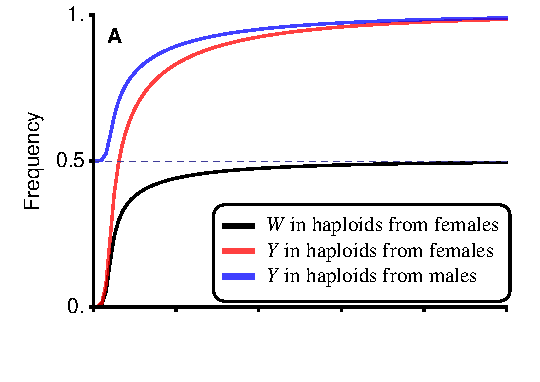
\includegraphics[width=0.5\linewidth]{FreqWLowR}\\
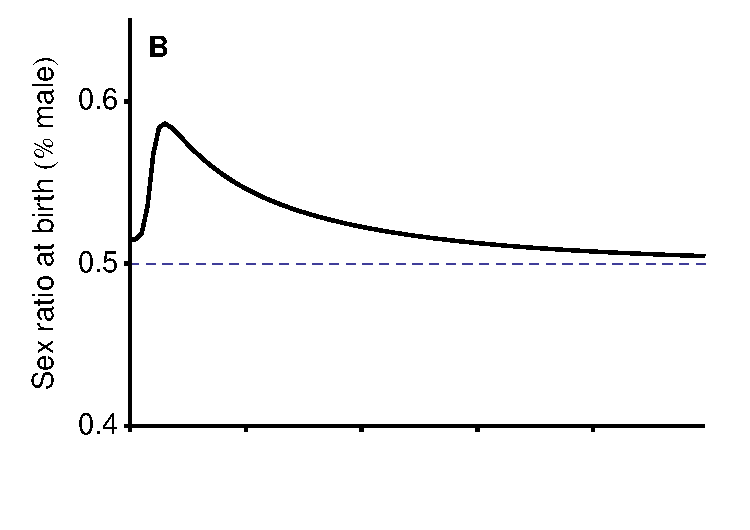
\includegraphics[width=0.5\linewidth]{SexRatioLowR}\\
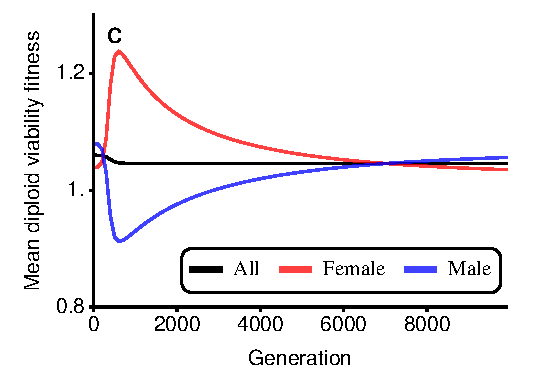
\includegraphics[width=0.5\linewidth]{MeanDipFitLowR}
\caption{
Haploid selection allows a neo-$W$ to invade an ancestral $XY$ system and fix (\textbf{A}) despite temporarily biasing the sex ratio further (\textbf{B}) and decreasing mean diploid viability fitness (\textbf{C}).
Complete turnover between genetic sex-determination systems occurs despite the neo-$W$ being less tightly linked to the selected locus than the ancestral sex-determining locus is, $R>r$.
Parameters: $k=1$, $s^f = 0.05$, $s^m = 0.15$, $h^f = h^m = 0.7$, $t^f = 0$, $t^m = -0.1$, $\alpha^m = \alpha^f = 1/2$, $r=0.01$, $R=0.05$.
}
\label{fig:WinvasionLowR}
\end{figure}
%%%%%%%%%%%%%%%%%%%%%%%%%%%%%%%%%%%%%%%%%%%%%%%%%%%%%%%%%

%%%%%%%%%%%%%%%%%%%%%%%%%%%%%%%%%%%%%%%%%%%%%%%%%%%%%%%%%
%W invades XY but does not fix
%%%%%%%%%%%%%%%%%%%%%%%%%%%%%%%%%%%%%%%%%%%%%%%%%%%%%%%%%
\begin{figure}
\centering
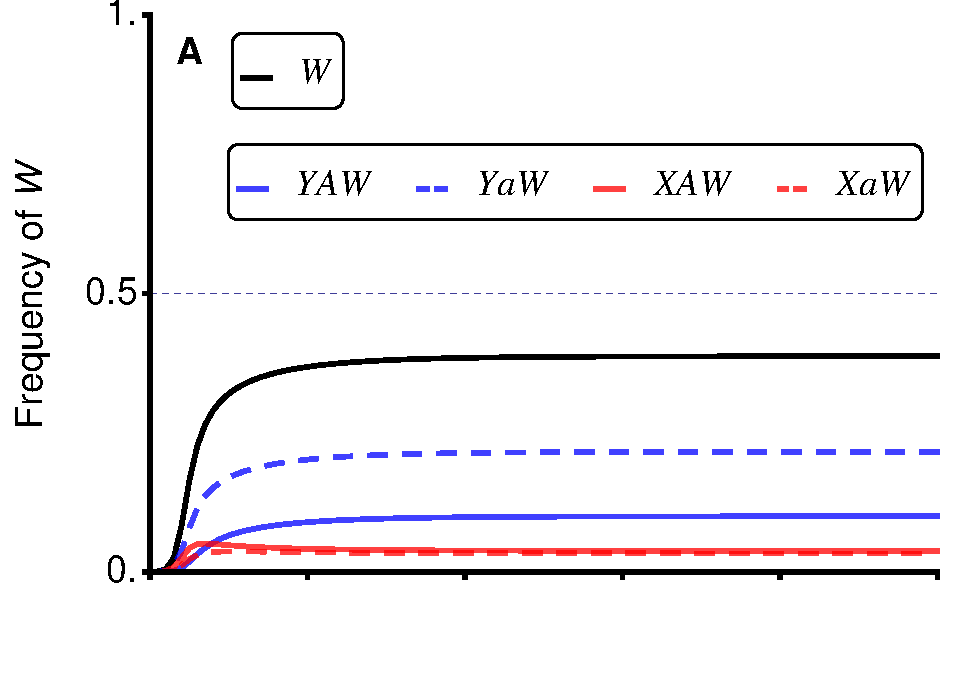
\includegraphics[width=0.5\linewidth]{FreqWHighR}\\
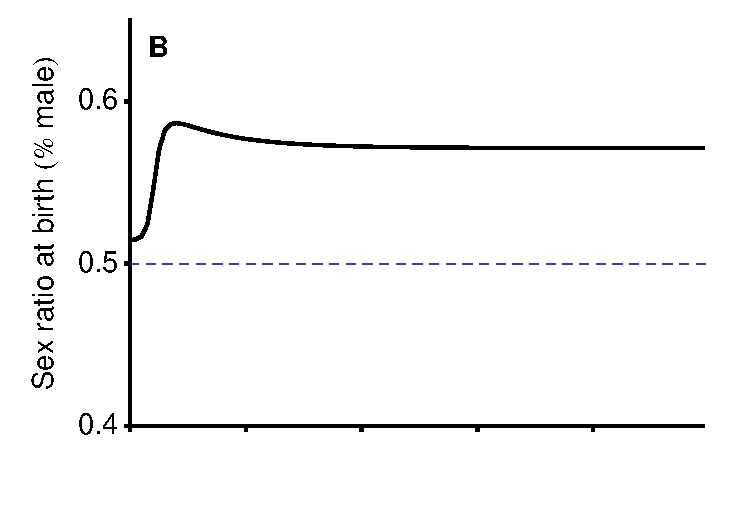
\includegraphics[width=0.5\linewidth]{SexRatioHighR}\\
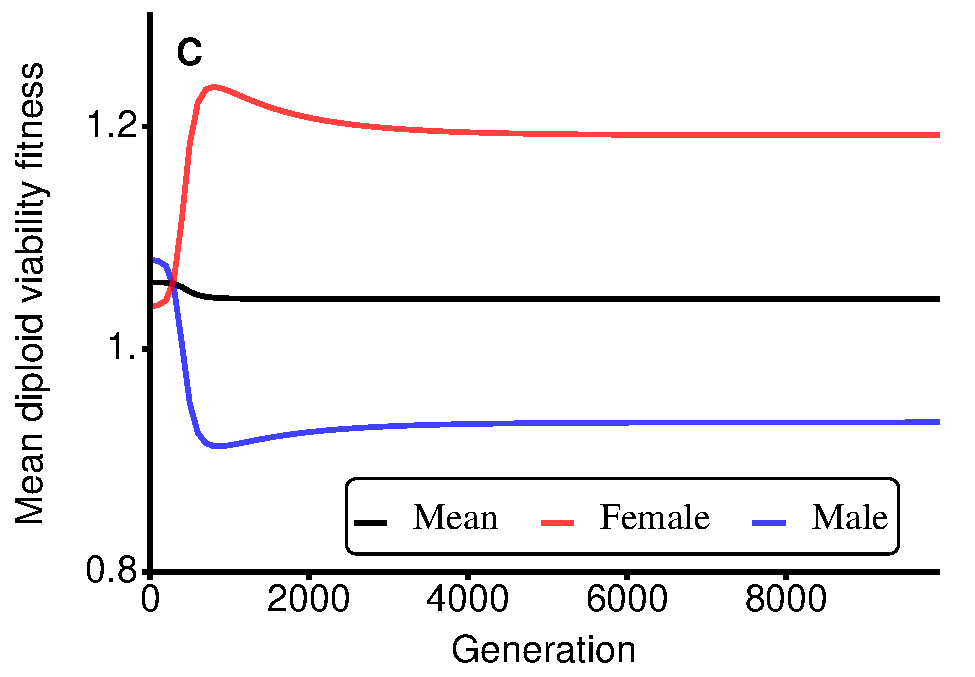
\includegraphics[width=0.5\linewidth]{MeanDipFitHighR}
\caption{
Haploid selection allows a completely unlinked neo-$W$ to invade an ancestral $XY$ system (\textbf{A}) despite further biasing the sex ratio (\textbf{B}) and decreasing mean diploid viability fitness (\textbf{C}).
The neo-$W$ does not fix (although variation at the \textbf{A} locus is maintained, $V_A>0$), resulting in a polymorphic sex-determination system.
Parameters as in Figure \ref{fig:WinvasionLowR} but with $R=0.5$.
}
\label{fig:WinvasionHighR}
\end{figure}
%%%%%%%%%%%%%%%%%%%%%%%%%%%%%%%%%%%%%%%%%%%%%%%%%%%%%%%%%

%%%%%%%%%%%%%%%%%%%%%%%%%%%%%%%%%%%%%%%%%%%%%%%%%%%%%%%%%
%W invades for all rates of recombination with selected locus
%%%%%%%%%%%%%%%%%%%%%%%%%%%%%%%%%%%%%%%%%%%%%%%%%%%%%%%%%
%\begin{figure}
%\centering
%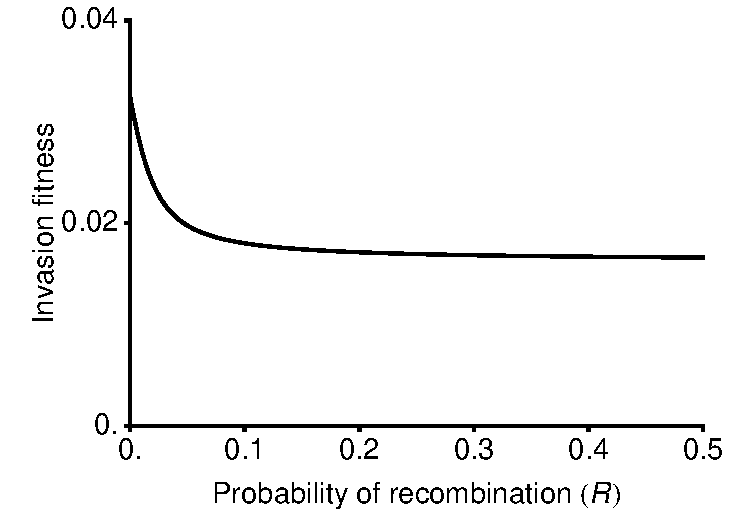
\includegraphics[width=0.5\linewidth]{InvasionVsRecombination}
%\caption{
%A neo-$W$ invades an ancestral $XY$ system with haploid selection regardless of how tightly it is linked to the selected locus. 
%Parameters as in Figure \ref{fig:WinvasionLowR}.
%}
%\label{fig:InvasionVsRecombination}
%\end{figure}
%%%%%%%%%%%%%%%%%%%%%%%%%%%%%%%%%%%%%%%%%%%%%%%%%%%%%%%%%

%%%%%%%%%%%%%%%%%%%%%%%%%%%%%%%%%%%%%%%%%%%%%%%%%%%%%%%%%
%W invasion versus position of selected locus
%%%%%%%%%%%%%%%%%%%%%%%%%%%%%%%%%%%%%%%%%%%%%%%%%%%%%%%%%
\begin{figure}
\centering
%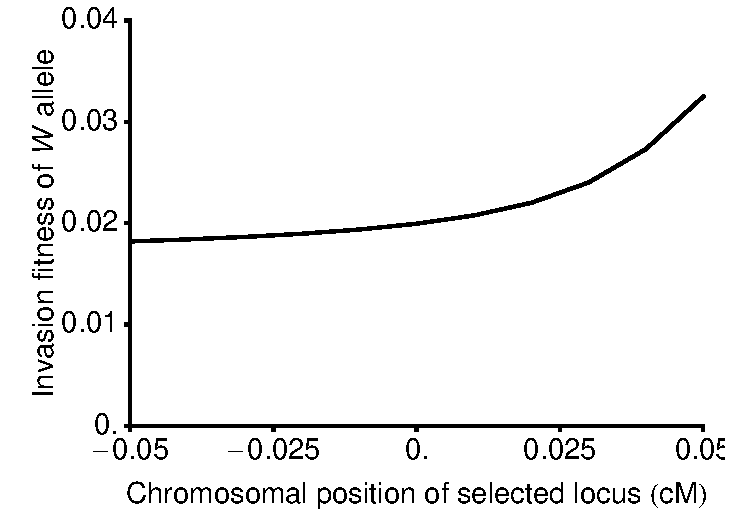
\includegraphics[width=0.5\linewidth]{InvasionVsCentiMorgans}
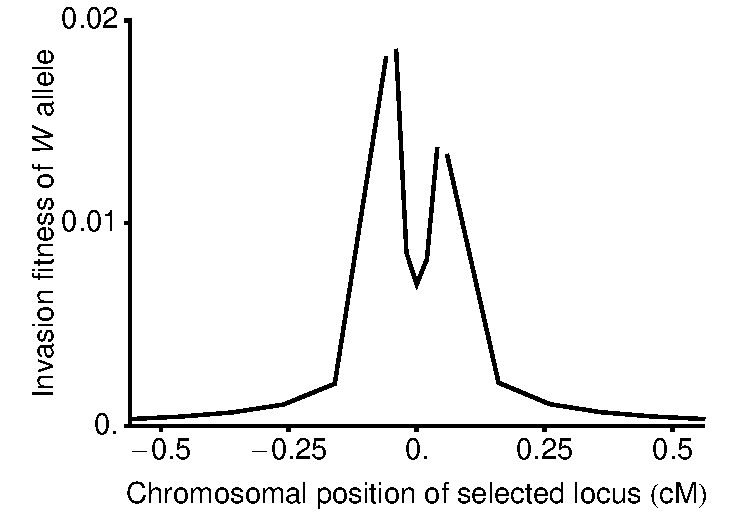
\includegraphics[width=0.5\linewidth]{InvasionVsCentiMorgansAllOrders}
\caption{
Haploid selection allows a neo-$W$ to invade an ancestral $XY$ system regardless of how tightly it and the ancestral sex-determining locus are linked to the selected locus. 
The ancestral sex-determining locus is located at -0.05 and the novel sex-determining locus is located at 0.05 (corresponding to the peaks of invasion fitness), such that the probability of a cross-over between them is $\approx0.1$.
The x-axis gives the position of the locus under haploid selection.
We used Haldane's map function \citep[Equation 3 in ][]{Haldane1919} to convert from map distance (centiMorgans) to the probability of a cross-over event. 
Parameters as in Figure \ref{fig:WinvasionLowR}.
}
\label{fig:InvasionVsCentiMorgans}
\end{figure}
%%%%%%%%%%%%%%%%%%%%%%%%%%%%%%%%%%%%%%%%%%%%%%%%%%%%%%%%%

%%%%%%%%%%%%%%%%%%%%%%%%%%%%%%%%%%%%%%%%%%%%%%%%%%%%%%%%%
%Y invades ZW and fixes (counter example to Kozi explanation)
%%%%%%%%%%%%%%%%%%%%%%%%%%%%%%%%%%%%%%%%%%%%%%%%%%%%%%%%%
\begin{figure}
\centering
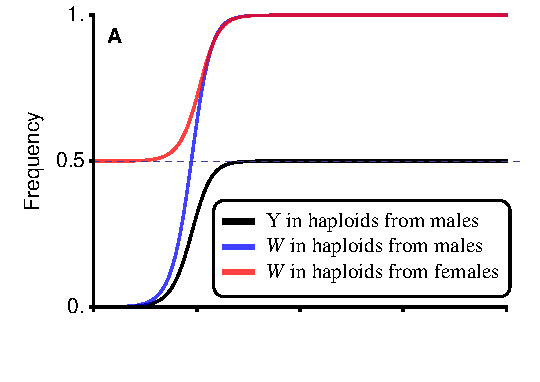
\includegraphics[width=0.5\linewidth]{FreqWCounterKozi}\\
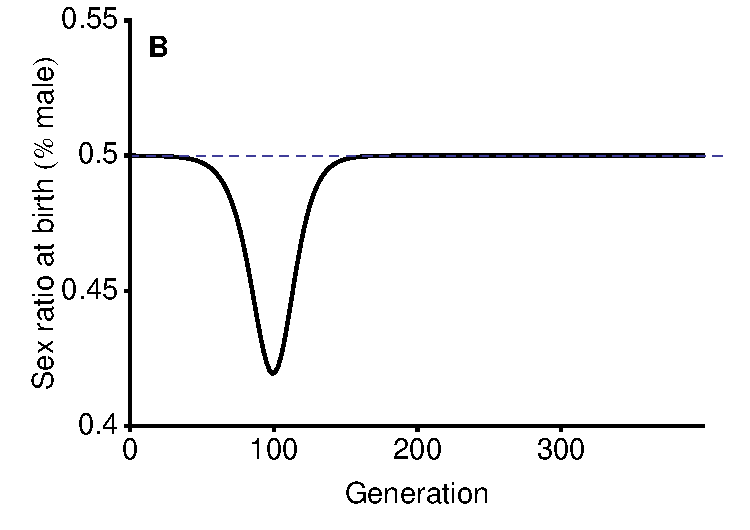
\includegraphics[width=0.5\linewidth]{SexRatioCounterKozi}\\
%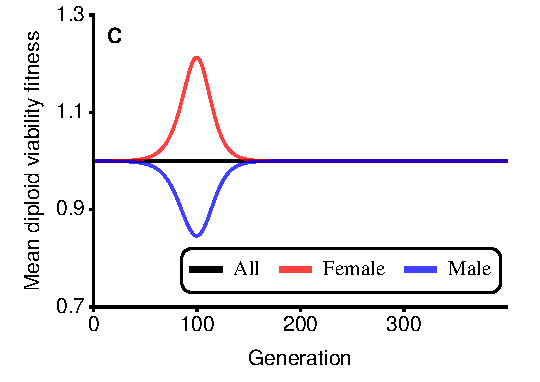
\includegraphics[width=0.5\linewidth]{MeanDipFitCounterKozi}
\caption{
Meiotic drive allows a neo-$Y$ to invade an ancestral $ZW$ system and fix (\textbf{A}) despite temporarily biasing the sex ratio (\textbf{B}). %and decreasing mean diploid viability fitness (\textbf{C}).
Parameters: $k=0$, $s^f = s^m = t^f = t^m = 0$, $\alpha^m = 0.4$, $\alpha^f = 1/2$, $r=0$, $R=0$.
}
\label{fig:CounterKozi}
\end{figure}
%%%%%%%%%%%%%%%%%%%%%%%%%%%%%%%%%%%%%%%%%%%%%%%%%%%%%%%%%

\end{document}



